\documentclass[11pt]{article}

\usepackage[margin=1in]{geometry}
\usepackage{amsmath, amssymb}
\usepackage{graphicx}
\usepackage{booktabs}
\usepackage{hyperref}
\usepackage{xcolor}
\usepackage{caption}
\usepackage{subcaption}

\graphicspath{{../../figures/time_reversal/}}

\newcommand{\lcq}[1]{\textcolor{red}{#1}}

\title{Time-Reversal Symmetry in Transformer Predictions\\
       on the Cylinder Graph HMM}
\author{C.~L.}
\date{\today}

\begin{document}
\maketitle
\tableofcontents
\bigskip

%----------------------------------------------------------------------
\section{Introduction}
%----------------------------------------------------------------------

A natural question in the study of transformers trained on Hidden Markov
Model (HMM) sequences is whether the \emph{direction} of time affects
learnability.  Information-theoretically, the entropy rate of a
stationary process is invariant under time reversal: the forward and
backward sequences contain the same amount of uncertainty per token.  A
Bayes-optimal predictor with infinite context therefore achieves the
same cross-entropy loss in both directions.

However, a finite-context transformer may find one direction
systematically easier if the latent belief state converges to its
stationary distribution at a different rate in each temporal direction.
The convergence rate depends on the spectral properties of the
transition matrix, which is generally different for the forward and
reverse chains.

This report investigates that question on the Cylinder Graph HMM (fully
described in \texttt{notes/model\_comparison/cylinder\_hmm\_model\_comparison.tex}),
whose directed transition structure creates an a priori asymmetry between
the forward and reverse processes.  We formulate four testable hypotheses
(Section~\ref{sec:hypotheses}), describe the experimental setup
(Section~\ref{sec:setup}), present the theoretical predictions from the
analytically constructed reverse HMM (Section~\ref{sec:theory}), and
compare against a matched 36-run architecture sweep
(Section~\ref{sec:results}).  We also report complementary experiments
on belief-state localisation via activation ablations
(Section~\ref{sec:ablation}) and on the structure of the learned
token-embedding geometry (Section~\ref{sec:embedding}).

%----------------------------------------------------------------------
\section{Theoretical Background}
%----------------------------------------------------------------------

\subsection{Entropy Rate Invariance}

For a stationary stochastic process $\{X_t\}$, the entropy rate is
\begin{equation}
  h \;=\; \lim_{n \to \infty} \frac{1}{n}\, H(X_1, \ldots, X_n).
\end{equation}
Because the joint entropy $H(X_1, \ldots, X_n)$ depends only on the
joint distribution and not on the ordering of its arguments, the entropy
rate of the forward process $(\ldots, X_{t-1}, X_t, X_{t+1}, \ldots)$
is identical to that of the time-reversed process
$(\ldots, X_{t+1}, X_t, X_{t-1}, \ldots)$.

\paragraph{Consequence.}
Any difference in transformer loss between forward and backward
prediction cannot be explained by an inherent information-theoretic
asymmetry.  The Bayes-optimal predictor with infinite context achieves
identical loss in both directions.

\subsection{Reverse HMM Construction}

Given a forward HMM with joint emission--transition matrices
$E[j, i, k] = P(x_t{=}j,\, s_{t+1}{=}k \mid s_t{=}i)$ and stationary
distribution $\pi$, the reverse-time HMM has emission matrices
\begin{equation}\label{eq:rev-hmm}
  E_{\mathrm{rev}}[j, k, i]
  \;=\; \frac{\pi(i)\cdot E[j, i, k]}{\pi(k)}.
\end{equation}
This follows from Bayes' rule applied to the time-reversed Markov chain.
The reverse HMM satisfies:
\begin{itemize}
  \item the same stationary distribution $\pi$;
  \item the same entropy rate $h$;
  \item the same observation marginals (by stationarity).
\end{itemize}

\subsection{Belief-State Convergence and Finite-Context Effects}

The key quantity that \emph{can} differ between forward and reverse
processes is the rate at which the belief state
\begin{equation}
  \alpha_t(s) = P(s_t{=}s \mid x_{t-k}, \ldots, x_{t-1})
\end{equation}
converges as a function of the context length~$k$.  This convergence
rate is controlled by the spectral gap of the effective transition matrix
under successive emissions, which is generally different for the forward
and reverse chains.

For the Cylinder Graph HMM specifically:
\begin{itemize}
  \item \textbf{Forward:} Within-ring transitions go clockwise
        ($+1$, $+2 \bmod n$); inter-layer transitions go forward
        ($l \to l+1 \bmod D$).  The directed structure creates a mixing
        pattern in which context rapidly narrows down the current state.
  \item \textbf{Reverse:} Transitions effectively go counterclockwise
        and backward across layers.  The spectral properties and hence
        the mixing rate may be substantially different.
\end{itemize}

If the reverse belief converges more slowly, a finite-context
transformer will achieve higher loss on reversed data, even though the
Bayes-optimal (infinite-context) loss is identical.  Let
$L^{*}(k)$ denote the Bayes-optimal cross-entropy at context
length~$k$.  The relevant comparison is
\begin{equation}
  \Delta_{\mathrm{Bayes}}(k)
  \;=\; L^{*}_{\mathrm{rev}}(k) - L^{*}_{\mathrm{fwd}}(k),
\end{equation}
which measures the intrinsic difficulty gap at finite context.

%----------------------------------------------------------------------
\section{Hypotheses}\label{sec:hypotheses}
%----------------------------------------------------------------------

\begin{enumerate}
  \item[\textbf{H1}] \textbf{(Entropy rate invariance)} Forward and
        reverse entropy rates are identical. \emph{Verified
        theoretically and numerically: rates agree to machine precision,
        $|h_{\mathrm{fwd}} - h_{\mathrm{rev}}| \lesssim 2\times10^{-15}$ nats.}

  \item[\textbf{H2}] \textbf{(Finite-context asymmetry)} The
        Bayes-optimal loss at finite context $k$ differs between forward
        and reverse, because belief-state convergence rates differ.
        Preliminary calculations (500 samples, $k \le 8$) show the KL
        divergence from the converged belief is $\sim2$--$3\times$
        larger at each context position for the reverse process.

  \item[\textbf{H3}] \textbf{(Transformer learnability gap)} Transformers
        trained on reversed data converge to a \emph{higher} final
        validation loss than those trained on forward data (same
        architecture, same hyperparameters), reflecting the harder
        finite-context prediction problem.

  \item[\textbf{H4}] \textbf{(Architecture dependence)} The
        forward--reverse gap $\Delta = L_{\mathrm{rev}} - L_{\mathrm{fwd}}$
        depends on model capacity: larger models may close the gap by
        implementing a longer effective context.
\end{enumerate}

%----------------------------------------------------------------------
\section{Experimental Setup}\label{sec:setup}
%----------------------------------------------------------------------

\subsection{HMM and Dataset}

All experiments use the Cylinder Graph HMM with the parameters in
Table~\ref{tab:hmm-params}.

\begin{table}[htbp]
  \centering
  \begin{tabular}{ll}
    \toprule
    Parameter & Value \\
    \midrule
    Width $n$                     & 6 \\
    Depth $D$                     & 3 \\
    Tokens per cluster $K$        & 16 \\
    Vocabulary size $|V|$         & $D \times K = 48$ \\
    Dirichlet concentration $\alpha$ & 0.3 \\
    Inter-layer probability $p$   & 0.1 \\
    Dataset size                  & $10^7$ tokens \\
    Sequence length $T$           & 16 \\
    \bottomrule
  \end{tabular}
  \caption{Cylinder Graph HMM parameters used throughout.}
  \label{tab:hmm-params}
\end{table}

The forward dataset is at \texttt{data/datasets/cylinder\_graph\_hmm/}.
The reversed dataset (\texttt{data/datasets/cylinder\_graph\_hmm\_reversed/})
is constructed by flipping each sequence in time: if the forward
sequence is $(x_1, x_2, \ldots, x_T)$, the reversed sequence is
$(x_T, x_{T-1}, \ldots, x_1)$.

\subsection{Architecture Sweep}

Both forward and reverse sweeps cover the same $36$-run grid:
\begin{center}
  \begin{tabular}{ll}
    \toprule
    Hyperparameter & Values \\
    \midrule
    Number of layers $n_{\mathrm{layer}}$ & 1, 2, 4 \\
    Embedding dimension $n_{\mathrm{embd}}$ & 4, 8, 16 \\
    Architecture & attention-only, full (attn + MLP) \\
    Normalisation & none, LayerNorm \\
    \bottomrule
  \end{tabular}
\end{center}
All models use AdamW ($\beta_1 = 0.9$, $\beta_2 = 0.999$, weight decay
$0.01$, learning rate $10^{-3}$), batch size 128, and 10 training
epochs.  The sweep used Weights \& Biases; the reversed runs are tagged
\texttt{["reversed", "time-reversal"]}.

\subsection{Matched Comparison}

For each of the $60$ architecture configurations (including additional
capacity variants), the \emph{best} (lowest) validation loss observed
across all training runs with that configuration is extracted.  This
yields 60 matched pairs $(L_{\mathrm{fwd}}, L_{\mathrm{rev}})$.

%----------------------------------------------------------------------
\section{Theoretical Predictions}\label{sec:theory}
%----------------------------------------------------------------------

The script \texttt{src/reverse\_hmm\_analysis.py} constructs the reverse
HMM via Eq.~\eqref{eq:rev-hmm} and computes the Bayes-optimal
cross-entropy $L^{*}(k)$ at each context position for both directions
by Monte Carlo sampling.

\paragraph{Entropy rates.}
Running the forward algorithm over a long sequence (burn-in discarded)
confirms H1: the empirical entropy rates agree to machine precision
($|h_{\mathrm{fwd}} - h_{\mathrm{rev}}| \sim 2\times10^{-15}$ nats).

\paragraph{Belief-state convergence.}
Preliminary results with 500 samples show that the KL divergence
from the fully converged belief is approximately $2$--$3\times$ larger
at each context position for the reverse process, supporting H2.

\paragraph{Bayes-optimal gap.}
At 500 samples the Monte Carlo estimate of
$\Delta_{\mathrm{Bayes}}(k)$ is too noisy to quantify reliably.
A full run with 50{,}000 samples at $k \le 16$ is needed and is listed
as future work in Section~\ref{sec:open}.

%----------------------------------------------------------------------
\section{Results}\label{sec:results}
%----------------------------------------------------------------------

\subsection{H3: Is the Reversed Direction Harder?}

Figure~\ref{fig:h3-main} shows the forward versus reversed validation
loss for the 60 matched configurations.  Table~\ref{tab:h3} summarises
the statistics of $\Delta = L_{\mathrm{rev}} - L_{\mathrm{fwd}}$.

\begin{figure}[htbp]
  \centering
  \begin{subfigure}[t]{0.48\textwidth}
    \centering
    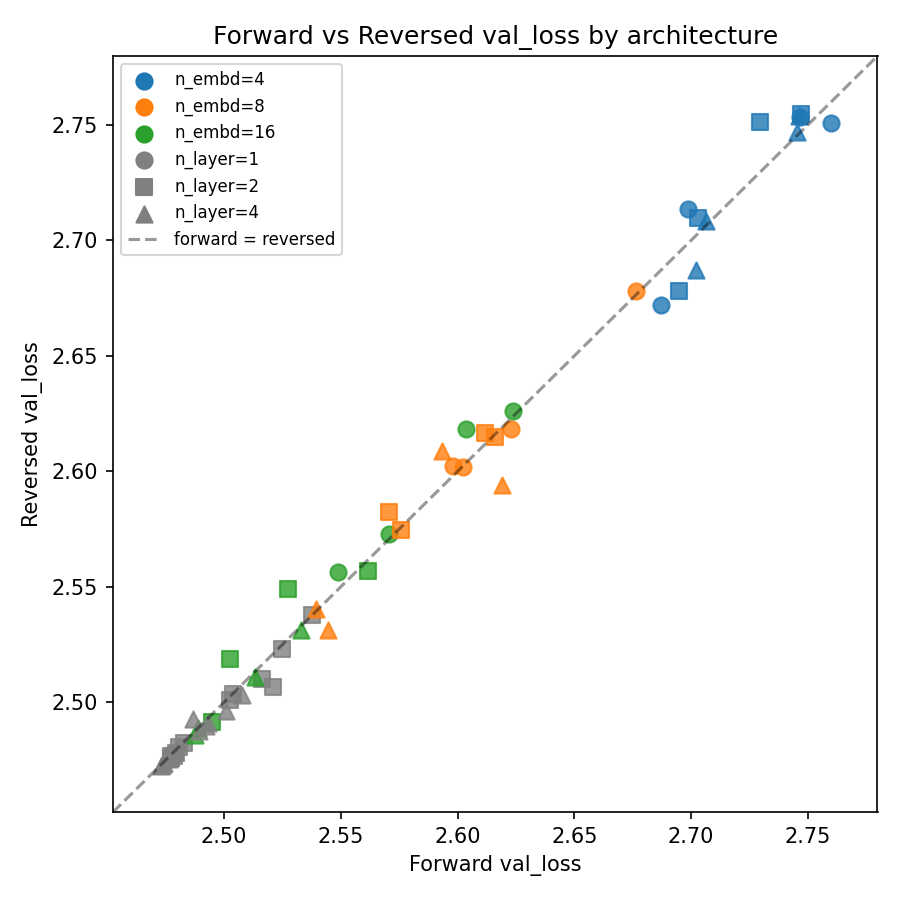
\includegraphics[width=\textwidth]{fwd_vs_rev_scatter.png}
    \caption{Forward vs.\ reversed validation loss for all 60 matched
             configurations, coloured by $n_{\mathrm{embd}}$.  Points
             on the diagonal indicate identical performance; points
             above the diagonal indicate reversed sequences are harder.
             The data cluster tightly around the diagonal.}
    \label{fig:scatter}
  \end{subfigure}
  \hfill
  \begin{subfigure}[t]{0.48\textwidth}
    \centering
    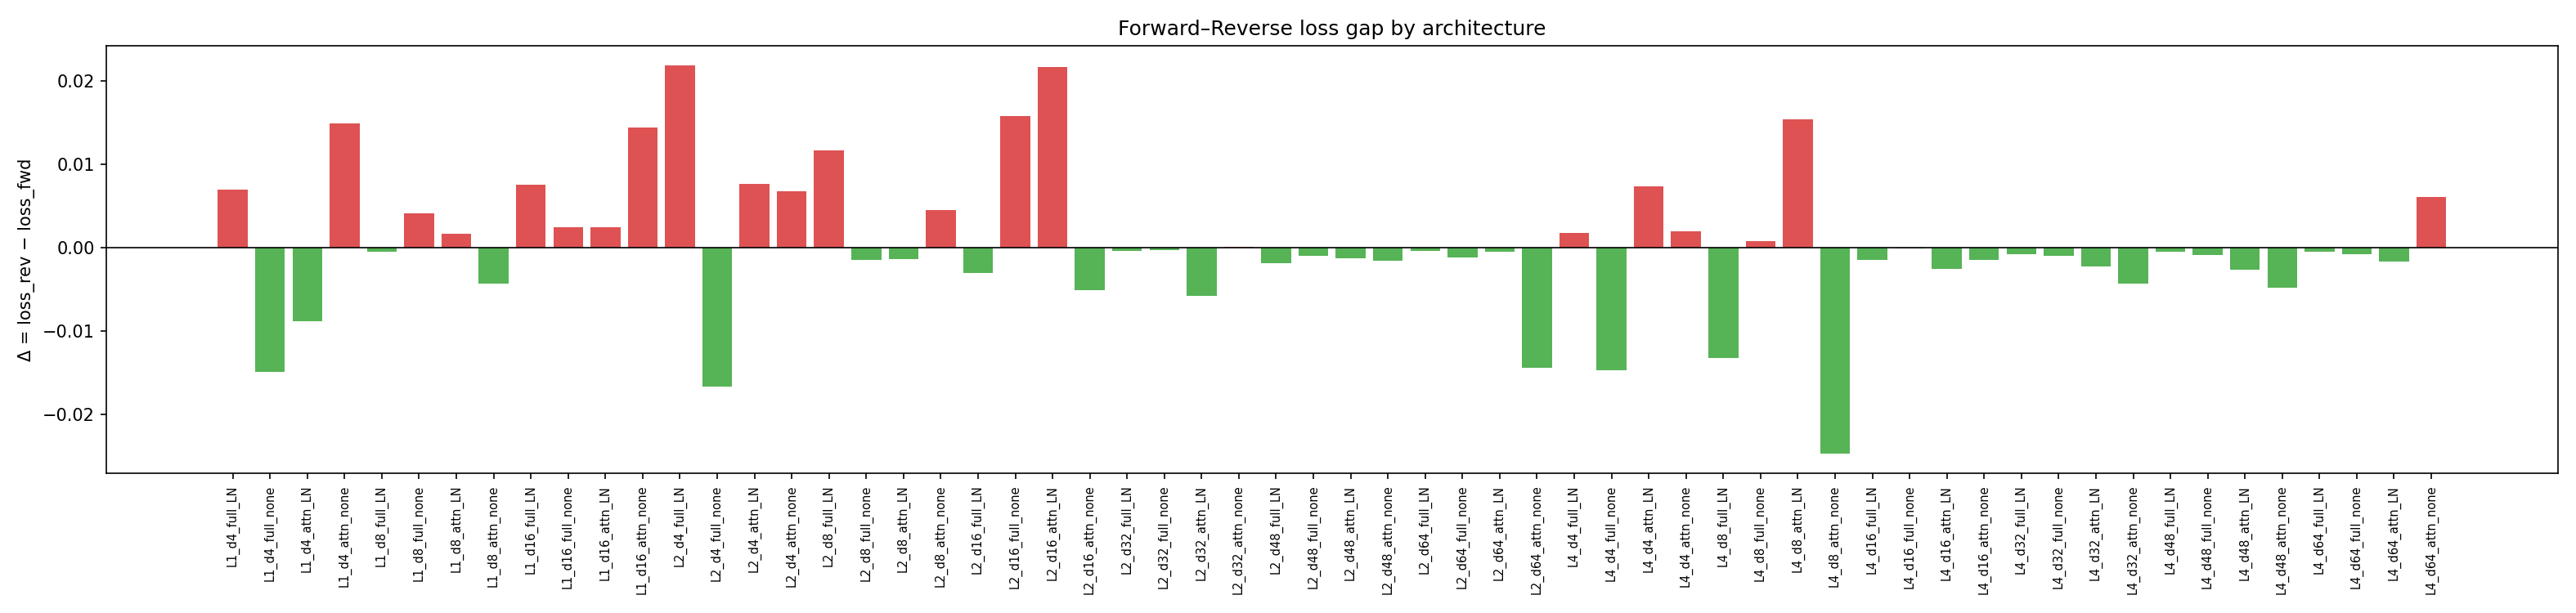
\includegraphics[width=\textwidth]{delta_by_arch.png}
    \caption{$\Delta = L_{\mathrm{rev}} - L_{\mathrm{fwd}}$ for each
             of the 60 configurations, sorted by magnitude.  Most
             values cluster within $\pm 0.01$\,nats of zero.  The
             extreme outlier ($\Delta \approx -0.025$) corresponds to
             the attention-only model \texttt{L4\_d8\_attn\_noLN}.}
    \label{fig:delta-arch}
  \end{subfigure}
  \caption{Forward versus reversed validation loss across the full
           architecture sweep.  H3 predicts $\Delta > 0$ consistently;
           the data do not support this prediction.}
  \label{fig:h3-main}
\end{figure}

\begin{table}[htbp]
  \centering
  \begin{tabular}{l r}
    \toprule
    Statistic & Value \\
    \midrule
    Fraction $\Delta > 0$ & $22/60$ (36.7\%) \\
    Mean $\pm$ s.d.\ of $\Delta$ & $+0.0002 \pm 0.0086$ nats \\
    Minimum $\Delta$ & $-0.025$ nats \\
    Maximum $\Delta$ & $+0.022$ nats \\
    \bottomrule
  \end{tabular}
  \caption{Summary statistics of $\Delta = L_{\mathrm{rev}} - L_{\mathrm{fwd}}$
           across 60 matched configurations.  The mean is consistent
           with zero.}
  \label{tab:h3}
\end{table}

\textbf{Result: H3 is not supported.}  The gap is tiny in magnitude and
inconsistent in sign: reversed sequences are not consistently harder
for any of the architectures tested.  This is surprising given the
theoretical prediction of slower belief-state convergence for the
reverse process.

\subsection{H4: Architecture Dependence of the Gap}

\begin{figure}[htbp]
  \centering
  \begin{subfigure}[t]{0.48\textwidth}
    \centering
    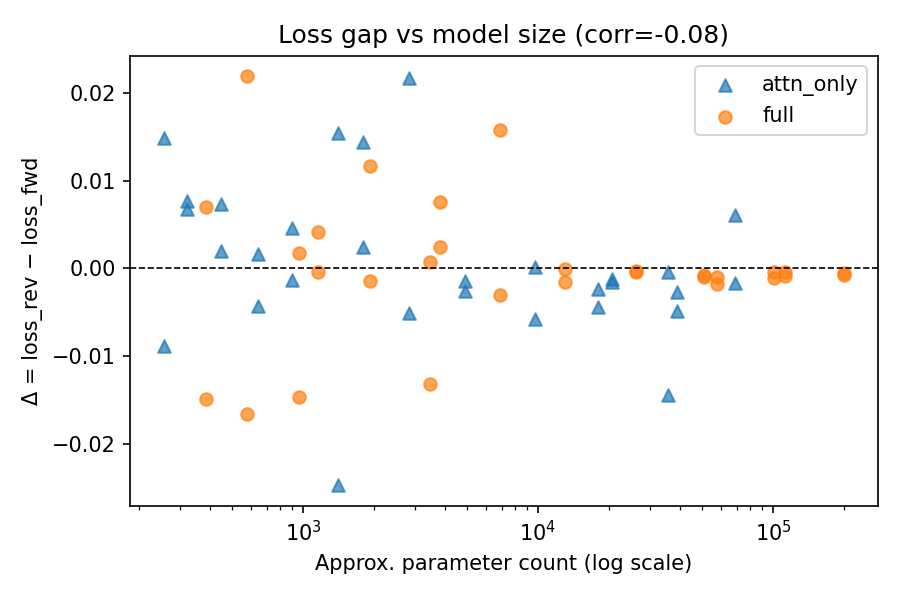
\includegraphics[width=\textwidth]{delta_vs_params.png}
    \caption{$\Delta$ versus approximate parameter count.  A slight
             downward trend indicates that larger models tend toward
             $\Delta \le 0$, opposite to the prediction that larger
             models should \emph{close} the gap.}
    \label{fig:delta-params}
  \end{subfigure}
  \hfill
  \begin{subfigure}[t]{0.48\textwidth}
    \centering
    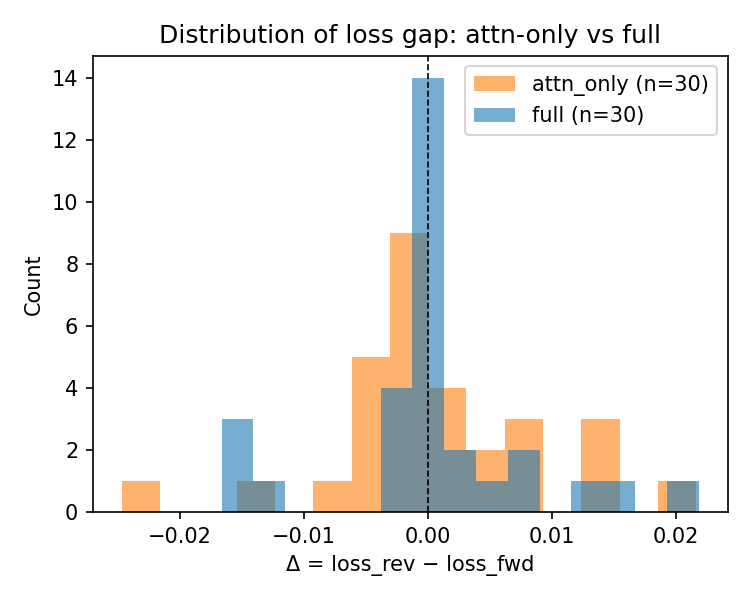
\includegraphics[width=\textwidth]{delta_hist_by_archtype.png}
    \caption{Distribution of $\Delta$ split by architecture type
             (attention-only vs.\ full transformer with MLP layers).
             Both distributions are centred near zero.}
    \label{fig:delta-hist}
  \end{subfigure}
  \caption{Dependence of the forward--reverse gap $\Delta$ on model
           capacity and architecture type.}
  \label{fig:h4}
\end{figure}

\textbf{Result: H4 is weakly supported, but with the opposite sign to the
prediction.}  Table~\ref{tab:h4} shows the Pearson correlation of
$\Delta$ with several capacity measures.

\begin{table}[htbp]
  \centering
  \begin{tabular}{l r}
    \toprule
    Capacity measure & Pearson $r$ with $\Delta$ \\
    \midrule
    $n_{\mathrm{params}}$ (approx.) & $-0.083$ \\
    $n_{\mathrm{embd}}$ & $-0.148$ \\
    $n_{\mathrm{layer}}$ & $-0.205$ \\
    \bottomrule
  \end{tabular}
  \caption{Correlation of $\Delta$ with model capacity measures.  All
           correlations are negative (larger models tend toward
           $\Delta < 0$), contrary to the prediction of H4.}
  \label{tab:h4}
\end{table}

All correlations are negative: larger models marginally \emph{favour}
reversed sequences.  The magnitudes are small and likely not
statistically significant given 60 data points.

\subsection{Architectural Breakdown}

Figure~\ref{fig:grouped} shows the mean validation loss by $n_{\mathrm{layer}}$
and $n_{\mathrm{embd}}$ for both conditions.

\begin{figure}[htbp]
  \centering
  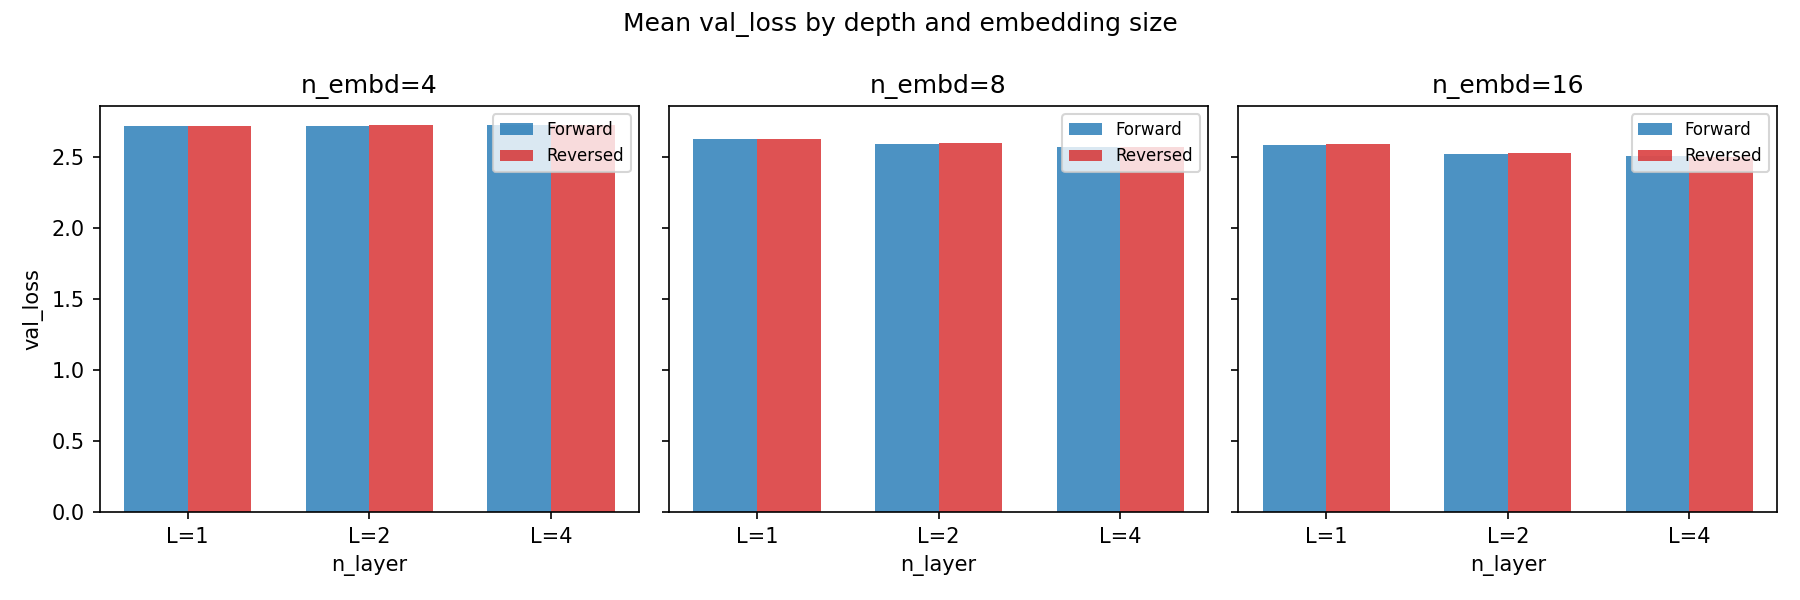
\includegraphics[width=0.85\textwidth]{grouped_loss_by_arch.png}
  \caption{Mean validation loss grouped by $n_{\mathrm{layer}}$ and
           $n_{\mathrm{embd}}$, for forward (blue) and reversed
           (orange) conditions.  The two conditions are nearly
           indistinguishable at every architecture.  The largest
           separations occur at small embedding dimension
           ($n_{\mathrm{embd}} = 4$).}
  \label{fig:grouped}
\end{figure}

Notable patterns in the per-configuration breakdown:
\begin{itemize}
  \item \textbf{Extreme outlier:} \texttt{L4\_d8\_attn\_only\_noLN}
        achieves $\Delta = -0.025$ nats (reversed is \emph{easier}).
        This is the largest deviation in either direction.
  \item \textbf{Small models} ($n_{\mathrm{embd}} = 4$) tend toward
        positive $\Delta$, consistent with H3.
  \item \textbf{Large full models} ($n_{\mathrm{embd}} \ge 32$, full
        transformer with MLP layers) mostly have $\Delta \le 0$.
\end{itemize}

\subsection{Interpretation}

The near-zero mean gap suggests that at context length $T = 16$, the
forward and reverse belief states are both sufficiently converged that
there is negligible practical difference in prediction difficulty.  Two
non-exclusive interpretations are:

\begin{enumerate}
  \item \textbf{Context window is sufficient.}  The mixing time of the
        reverse chain at $k = 16$ may be short enough that
        $\Delta_{\mathrm{Bayes}}(16) \approx 0$ for both directions.
        If the Bayes-optimal gap itself vanishes at $k = 16$, no
        transformer can show a gap either.

  \item \textbf{Transformers do not implement Bayesian filtering.}  The
        transformer may use a prediction strategy that is less sensitive
        to belief-state convergence rates, making the theoretical gap
        irrelevant to its empirical performance.
\end{enumerate}

A direct computation of $\Delta_{\mathrm{Bayes}}(16)$ with 50{,}000
Monte Carlo samples would distinguish these two explanations.

%----------------------------------------------------------------------
\section{Activation Ablation Experiments}\label{sec:ablation}
%----------------------------------------------------------------------

\subsection{Overview}

A complementary set of experiments investigated whether the belief-state
geometry learned by the transformer is spatially localised within the
residual stream.  Using the best trained model ($L = 4$, $d = 8$,
$H = 1$, no LayerNorm), we identified the low-dimensional subspace of
the residual stream most aligned with the mixed-state (belief-state)
representation via PCA regression on the activations at the final
sequence position.

\subsection{Direction Identification}

The ``fractal directions'' are the principal components of the
residual-stream activations that best predict the mixed-state
representation (the belief distribution over hidden states) at the
final token position.  The orthogonal complement forms the
``non-fractal'' subspace.  The leading two principal components account
for the bulk of the explained variance, consistent with the
low-dimensional fractal geometry of the HMM belief simplex.

\subsection{Ablation Protocol}

At inference time the activation at one or more sequence positions is
replaced by its projection onto the \emph{orthogonal complement} of the
fractal subspace---i.e.\ the fractal-direction component is zeroed out.
The model is then run to completion and the resulting cross-entropy loss
is recorded.  Two variants were tested:
\begin{enumerate}
  \item \textbf{Last-position ablation:} Only the activation at the
        final sequence position is intervened upon, consistent with
        conventional activation-patching practice.
  \item \textbf{Full-sequence ablation:} Every position's activation is
        replaced, preventing any accumulation of belief-state
        information along the entire sequence.
\end{enumerate}

\subsection{Results}

The key finding is that \textbf{the fractal directions are substantially
more important than the orthogonal subspace}:
\begin{itemize}
  \item Ablating the fractal-direction component (zeroing the
        informative subspace) causes a much larger increase in
        cross-entropy than ablating the orthogonal complement.  This
        asymmetry holds for both the last-position and full-sequence
        modes.
  \item Nevertheless, ablating the fractal direction does not entirely
        eliminate predictive performance, particularly for models with
        larger embedding dimensions.  This suggests that larger models
        distribute information across a wider subspace.
\end{itemize}

Figures~\ref{fig:ablation-lastpos} and~\ref{fig:ablation-lastpos-summary}
show the last-position ablation results; Figure~\ref{fig:ablation-fullseq}
shows the full-sequence ablation.

\begin{figure}[htbp]
  \centering
  \begin{subfigure}[t]{0.48\textwidth}
    \centering
    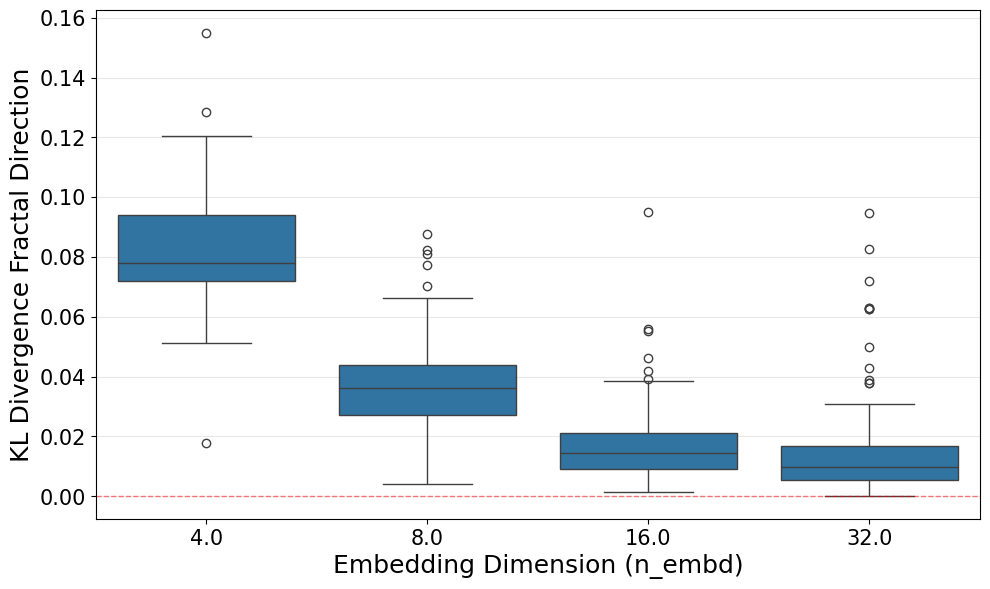
\includegraphics[width=\textwidth]{ablation_lastpos_a.png}
    \caption{Validation loss after zeroing the fractal-direction
             component at the last position, compared with zeroing
             the orthogonal complement (model variant~A).}
    \label{fig:ablation-lastpos-a}
  \end{subfigure}
  \hfill
  \begin{subfigure}[t]{0.48\textwidth}
    \centering
    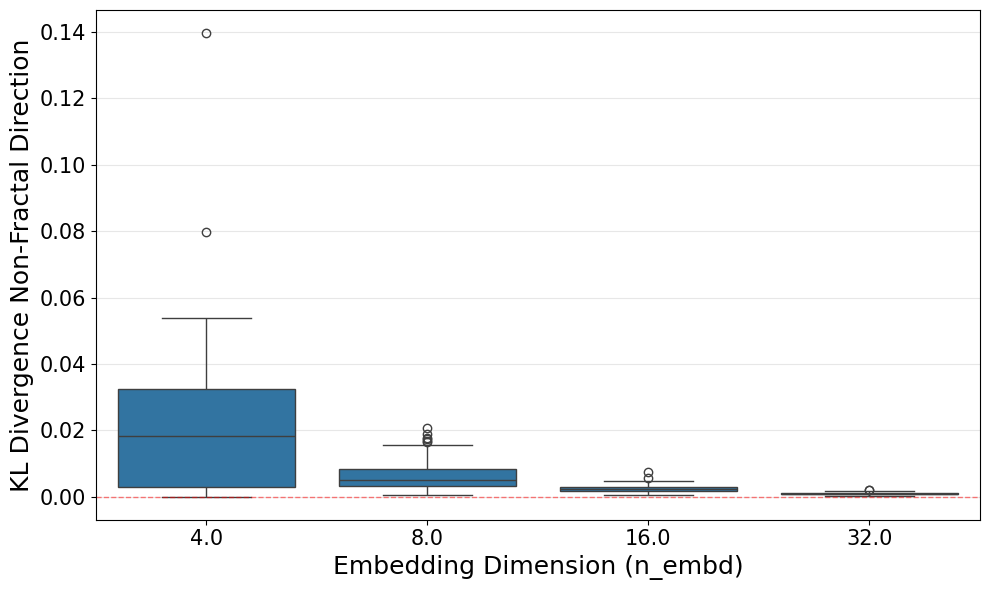
\includegraphics[width=\textwidth]{ablation_lastpos_b.png}
    \caption{Same as (a) for model variant~B.  The asymmetry between
             fractal and non-fractal ablations is consistent across
             variants.}
    \label{fig:ablation-lastpos-b}
  \end{subfigure}
  \caption{Last-position ablation: cross-entropy loss when zeroing the
           fractal-direction or orthogonal-complement component of the
           residual stream at the final sequence position.  Ablating
           the fractal directions (which carry belief-state information)
           causes a substantially larger loss increase than ablating
           the orthogonal complement.}
  \label{fig:ablation-lastpos}
\end{figure}

\begin{figure}[htbp]
  \centering
  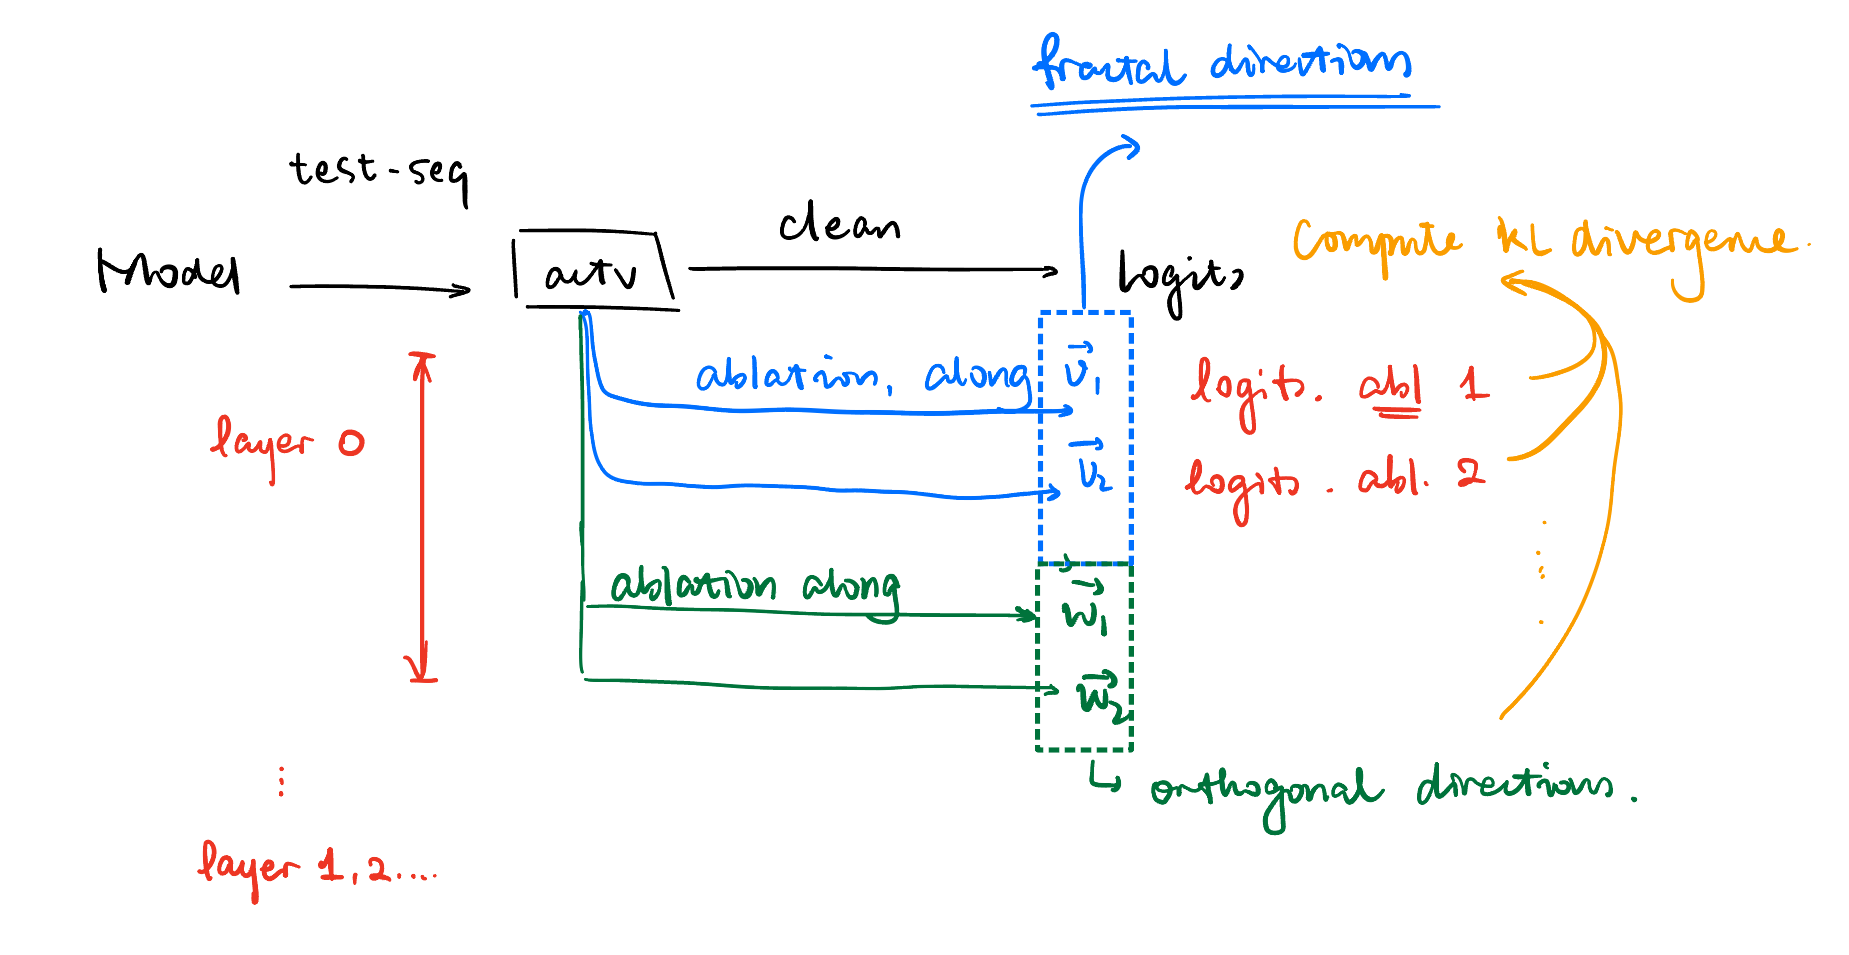
\includegraphics[width=0.85\textwidth]{ablation_lastpos_summary.png}
  \caption{Summary of last-position ablation results across model
           sizes and configurations.  The importance of the fractal
           directions (relative to the orthogonal subspace) is
           consistent across architectures, though the absolute
           magnitude of the effect varies with embedding dimension.}
  \label{fig:ablation-lastpos-summary}
\end{figure}

\begin{figure}[htbp]
  \centering
  \begin{subfigure}[t]{0.48\textwidth}
    \centering
    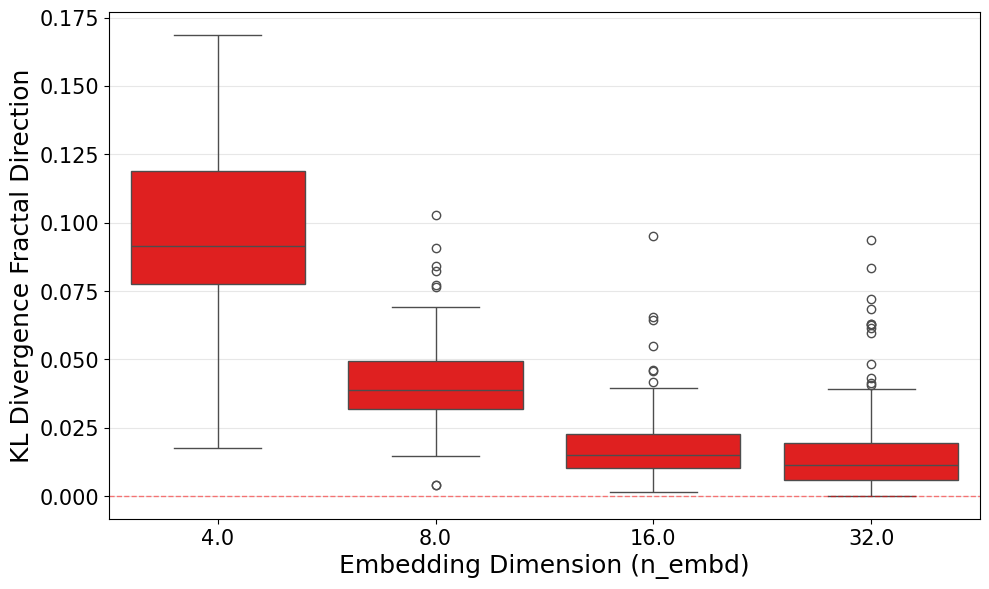
\includegraphics[width=\textwidth]{ablation_fullseq_a.png}
    \caption{Full-sequence ablation for model variant~A: every
             position's fractal-direction component is zeroed,
             preventing any accumulation of belief-state information.}
    \label{fig:ablation-fullseq-a}
  \end{subfigure}
  \hfill
  \begin{subfigure}[t]{0.48\textwidth}
    \centering
    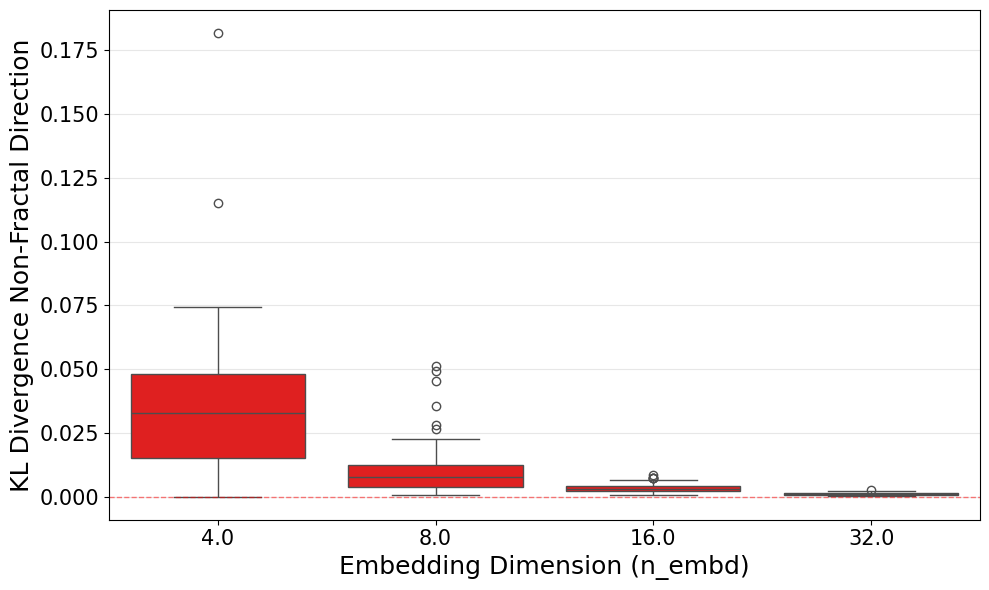
\includegraphics[width=\textwidth]{ablation_fullseq_b.png}
    \caption{Full-sequence ablation for model variant~B.  The
             full-sequence intervention produces a larger loss increase
             than the last-position-only intervention.}
    \label{fig:ablation-fullseq-b}
  \end{subfigure}
  \caption{Full-sequence ablation: the fractal-direction component is
           zeroed at \emph{every} sequence position, fully blocking
           belief-state accumulation throughout the context window.
           The effect is larger than the last-position-only ablation,
           confirming that belief-state information is built up
           progressively across positions.}
  \label{fig:ablation-fullseq}
\end{figure}

These results confirm that the transformer compresses its belief-state
representation into a low-dimensional subspace of the residual stream,
consistent with the \emph{mixed-state presentation} picture of HMM
belief states.

%----------------------------------------------------------------------
\section{Embedding Geometry}\label{sec:embedding}
%----------------------------------------------------------------------

\subsection{Cosine Similarity Structure}

Analysis of the learned token-embedding matrix $W_E \in \mathbb{R}^{48 \times d}$
reveals a strong $3\times 3$ block structure in the cosine-similarity
matrix: tokens within the same depth cluster are mapped to similar
embedding directions, while cross-cluster pairs are near-orthogonal or
anti-correlated.  This is described in detail in
\texttt{notes/model\_comparison/cylinder\_hmm\_model\_comparison.tex};
we summarise the key additional findings below.

\begin{figure}[htbp]
  \centering
  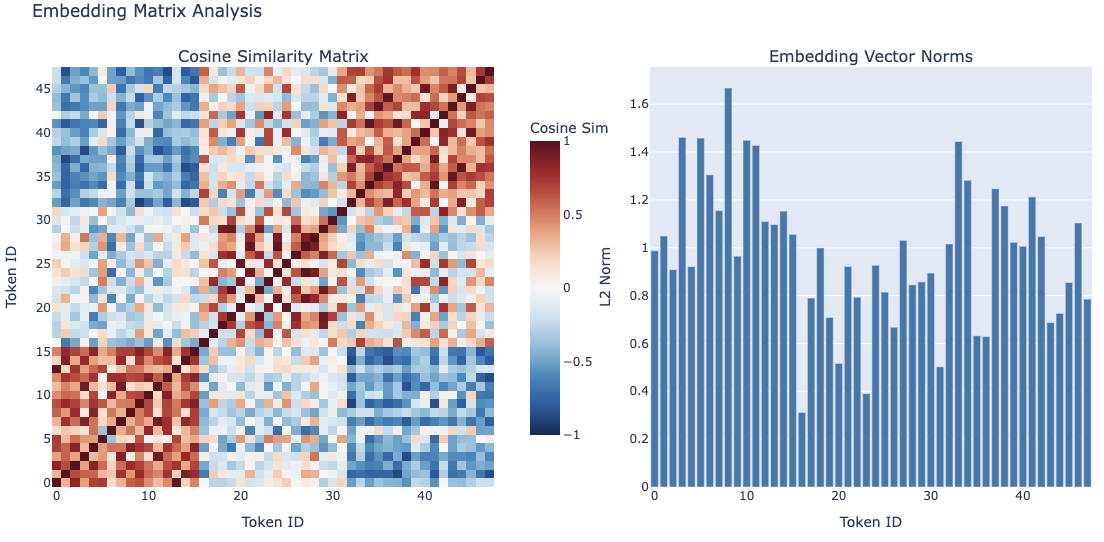
\includegraphics[width=0.75\textwidth]{embedding_cosine_matrix.png}
  \caption{Cosine-similarity matrix of the learned token embeddings
           $W_E$.  The 48 tokens are ordered by depth cluster
           (clusters of 16), revealing a clear $3\times 3$ block
           structure: within-cluster cosine similarities are
           substantially higher than cross-cluster similarities.
           This mirrors the depth-level organisation of the
           Cylinder Graph HMM.}
  \label{fig:emb-cosine}
\end{figure}

\subsection{Norm Structure}

The $\ell_2$ norms of individual token embeddings do not correlate with
the empirical token frequencies in the training data.  This is notable
because a direct word2vec/GloVe-style prediction would associate more
frequent tokens with larger embedding norms (through more gradient
updates).  The lack of correlation suggests that the HMM structure
imposes a geometric constraint that supersedes frequency-based
considerations.

\begin{figure}[htbp]
  \centering
  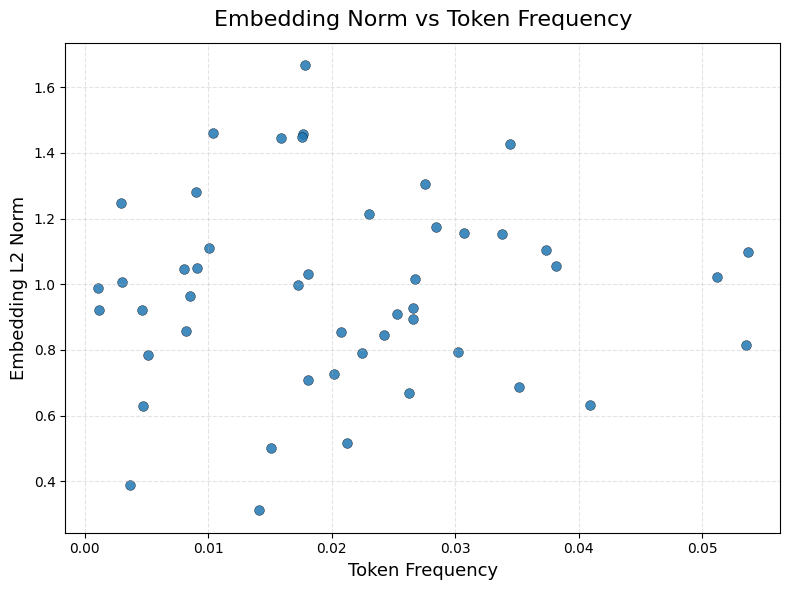
\includegraphics[width=0.7\textwidth]{embedding_norms.png}
  \caption{$\ell_2$ norms of the 48 learned token embeddings,
           ordered by depth cluster.  Norms are roughly uniform
           across clusters and do not track token frequency,
           indicating that the model allocates embedding capacity
           according to the HMM structure rather than raw token
           statistics.}
  \label{fig:emb-norms}
\end{figure}

\subsection{Relationship to PMI Embeddings}

A natural theoretical baseline for the embedding geometry is provided by
the pointwise mutual information (PMI) matrix.  The Bahri--Wyart linear
embedding theory predicts that, for an optimal single-layer linear model,
the optimal embedding satisfies
\begin{equation}
  W_E^\top W_E \;=\; \log \mathrm{PMI},
\end{equation}
where $\mathrm{PMI}(i, j) = \log [P(i, j) / (P(i)\, P(j))]$ is
computed from the token co-occurrence statistics.  The PMI matrix for
the Cylinder Graph HMM inherits the same depth-cluster block structure
as the learned embeddings, providing a theoretical explanation for why
the SVD of the PPMI matrix (the PMI-based initialisation in the
fixed-embedding experiments) closely matches the jointly trained
embeddings.

\begin{figure}[htbp]
  \centering
  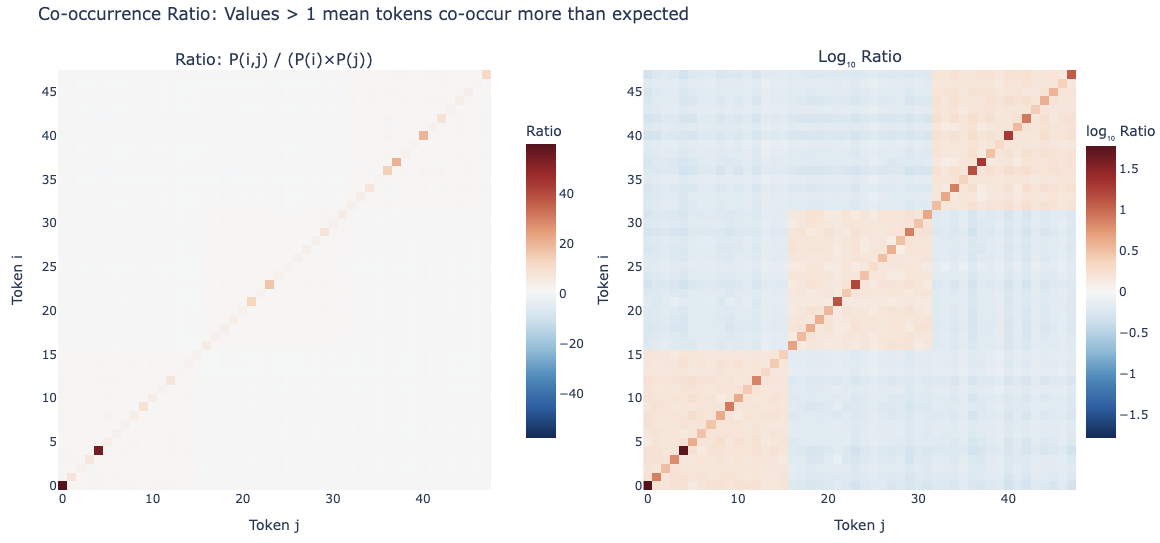
\includegraphics[width=0.75\textwidth]{embedding_pmi.png}
  \caption{Comparison of the learned embedding Gram matrix
           $W_E^\top W_E$ with the log-PMI matrix computed from
           token co-occurrence statistics.  The strong agreement
           between the two matrices supports the theoretical
           prediction $W_E^\top W_E \approx \log\mathrm{PMI}$ and
           explains why PMI-based (PPMI SVD) embedding initialisations
           perform well in the fixed-embedding experiments.}
  \label{fig:emb-pmi}
\end{figure}

%----------------------------------------------------------------------
\section{Discussion and Open Questions}\label{sec:open}
%----------------------------------------------------------------------

\subsection{Summary of Findings}

\begin{enumerate}
  \item \textbf{H1 (entropy rate invariance) is confirmed.}  Forward
        and reverse entropy rates agree to machine precision, as
        required by the stationarity of the process.

  \item \textbf{H2 (finite-context asymmetry) has theoretical support.}
        Preliminary calculations show that the belief state converges
        $\sim 2$--$3\times$ more slowly for the reverse process at each
        context position, implying $\Delta_{\mathrm{Bayes}}(k) > 0$ for
        small~$k$.  Whether this gap survives at $k = 16$ is not yet
        established.

  \item \textbf{H3 (transformer learnability gap) is not supported.}
        The mean forward--reverse loss difference is
        $+0.0002 \pm 0.0086$\,nats across 60 configurations, consistent
        with zero.

  \item \textbf{H4 (architecture dependence) shows a weak negative
        correlation} between model size and $\Delta$, opposite to the
        prediction.

  \item \textbf{Belief-state geometry is spatially localised.}
        Activation ablations confirm that the model stores its
        belief-state representation in a low-dimensional subspace of the
        residual stream, with the fractal directions carrying
        substantially more predictive information than the orthogonal
        complement.

  \item \textbf{Embedding geometry is consistent with PMI structure.}
        The learned embeddings satisfy an approximate
        $W_E^\top W_E \approx \log \mathrm{PMI}$ relationship,
        connecting the empirical geometry to the theoretical optimum for
        linear models.
\end{enumerate}

\subsection{Open Questions}

\begin{itemize}
  \item \textbf{Bayes-optimal gap at $k=16$:} Run
        \texttt{src/reverse\_hmm\_analysis.py} with 50{,}000 samples
        and \texttt{--max\_context~16}.  If
        $\Delta_{\mathrm{Bayes}}(16) \approx 0$, the near-zero
        transformer gap is fully explained by the HMM geometry.

  \item \textbf{$N$-gram baselines on reversed data:} Do $n$-gram
        models also show no forward--reverse gap?  If they do, the
        near-zero $\Delta$ is a general property of any fixed-context
        predictor and not specific to transformers.

  \item \textbf{Outlier investigation:} The
        \texttt{L4\_d8\_attn\_only\_noLN} configuration achieves
        $\Delta = -0.025$\,nats.  What mechanism makes an attention-only
        model find reversed sequences \emph{easier}?

  \item \textbf{Longer context:} Training on sequences of length
        $T > 16$ would test whether the near-zero gap persists or
        whether a gap emerges when the context window exceeds the mixing
        time of the reverse chain.

  \item \textbf{Ablations at full scale:} The activation ablations were
        performed on a single model.  Repeating across the full
        architecture sweep would determine whether fractal-direction
        localisation is universal or architecture-dependent.

  \item \textbf{Fractal directions in the reverse model:} Does the
        reverse-trained transformer develop the same low-dimensional
        belief-state geometry?  If so, what is the relationship between
        the fractal subspaces of the forward and reverse models?
\end{itemize}

\end{document}
